\section{Functionality description}
\label{sec:usermanual_func}
The Robotic Control Testbed is a Mobile Robot built from a commercial robot base with added funcionality.
The robot base consists of a four wheel vehicle with position and speed control embedded, integrated power and control
electronics and 16 ultrasonic sensors that give readings on the distance to close obstacles. Additionally front and
rear bumpers have been installed for safeguarding the robot while operating it
in very constrained areas and for manual stopping.

The Laser range reader can measure distances from 8mm up to 80m, depending on configuration. Typically it will function
with a resolution of 1mm and a range of 8mm to 8m. It is the main sensor along with the odometer readings in SLAM
navigation. It can be rotated with the servo to make three dimensional maps. The mechanism operates in open loop
mode, which gives a low precision angular rotation, given the mechanical hystheresys and the thermal and age deviations
of set.

Next to the laser the I/O board, or data acquisition board, is a general purpose input output board that connects to a compass, a two axis accelerometer,
the servo that controls the laser's tilt movement, and two current and voltage sensors one for monitoring the consumption of the robot base and the other for the power board and related devices. These sensors and actuators are controlled through the I/O board module.

For outdoor applications there is a global absolute position sensor which consists of a GPS antenna,
Radio receiver and battery for receiving differential corrections from a base station and a GPS receiver that
processes the data and converts it to an easier format readable by the onboard computer.

Vision applications can make use of the binocular camera, that in combination with the wrist, which gives pan and
tilt movement to the camera with respect to the robot base and is located on top of the laser, can direct the
focus of the attention in almost any direction. The wrist is internally controlled in position, speed and acceleration,
which gives precise and accurate motion control to the camera.

The onboard computer runs a full capable operating system and is the communications hub for controlling remotely
all the devices on the robot. Software controlling the devices may be installed onboard or in a remote computer.

\subsection{Visual identification of devices}


\begin{figure}[ht]
\centering
 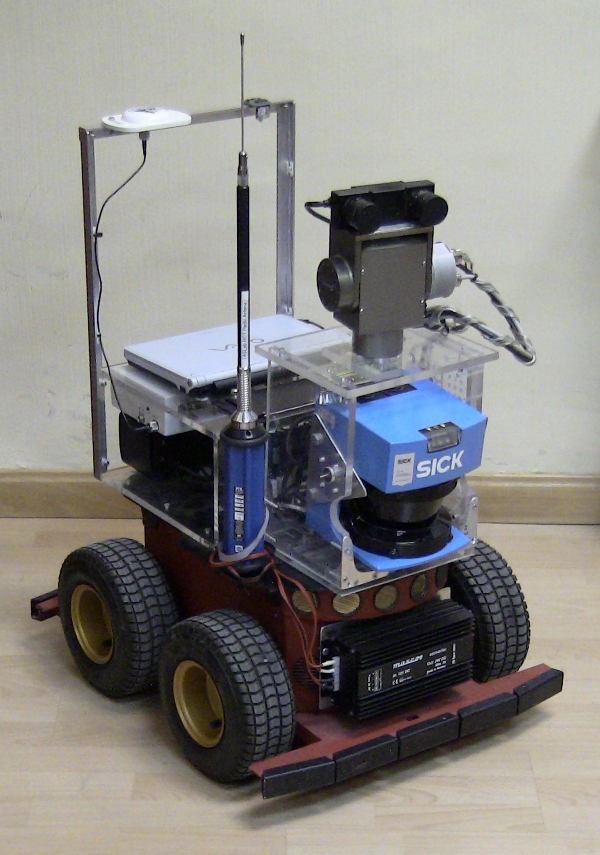
\includegraphics[width=0.4\textwidth]{figures/device_photos/higgs.jpg}
\caption{General view of Higgs.}
\end{figure}

\begin{figure}[ht]
\centering
 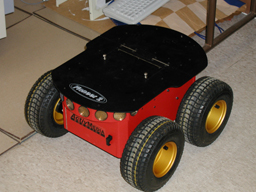
\includegraphics[width=0.4\textwidth]{figures/device_photos/p2at.jpg}
\caption{Robotic base Pioneer 2AT.}
\end{figure}

\begin{figure}[ht]
\centering
 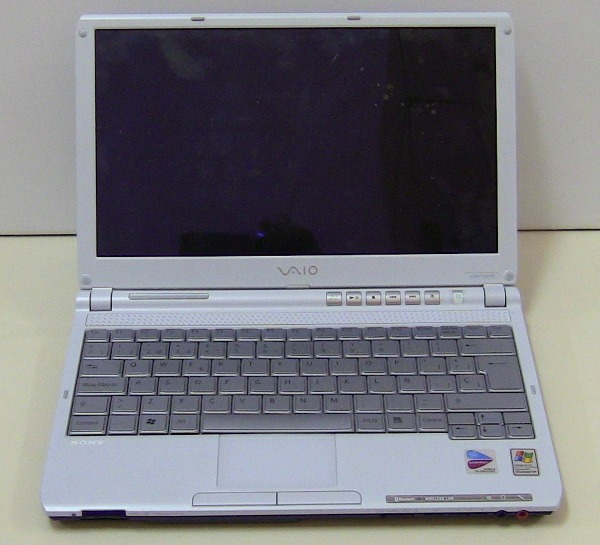
\includegraphics[width=0.3\textwidth]{figures/device_photos/vaio.jpg}
\caption{On board computer: VAIO laptop.}
\end{figure}

\begin{figure}[ht]
\centering
 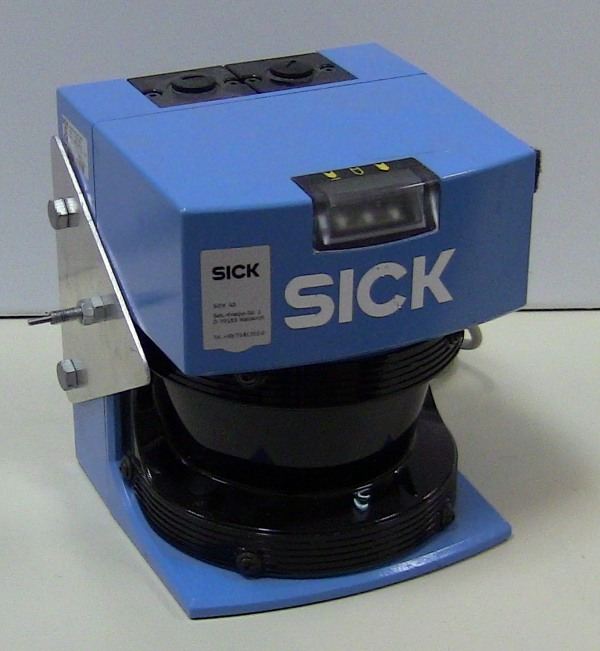
\includegraphics[width=0.3\textwidth]{figures/device_photos/laser.jpg}
\caption{Laser sensor.}
\end{figure}

\begin{figure}[ht]
\centering
 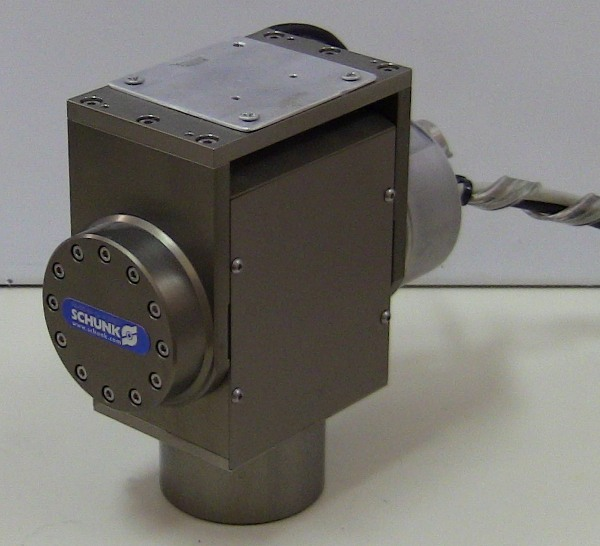
\includegraphics[width=0.4\textwidth]{figures/device_photos/wrist.jpg}
\caption{Wrist.}
\end{figure}

\begin{figure}[ht]
\centering
 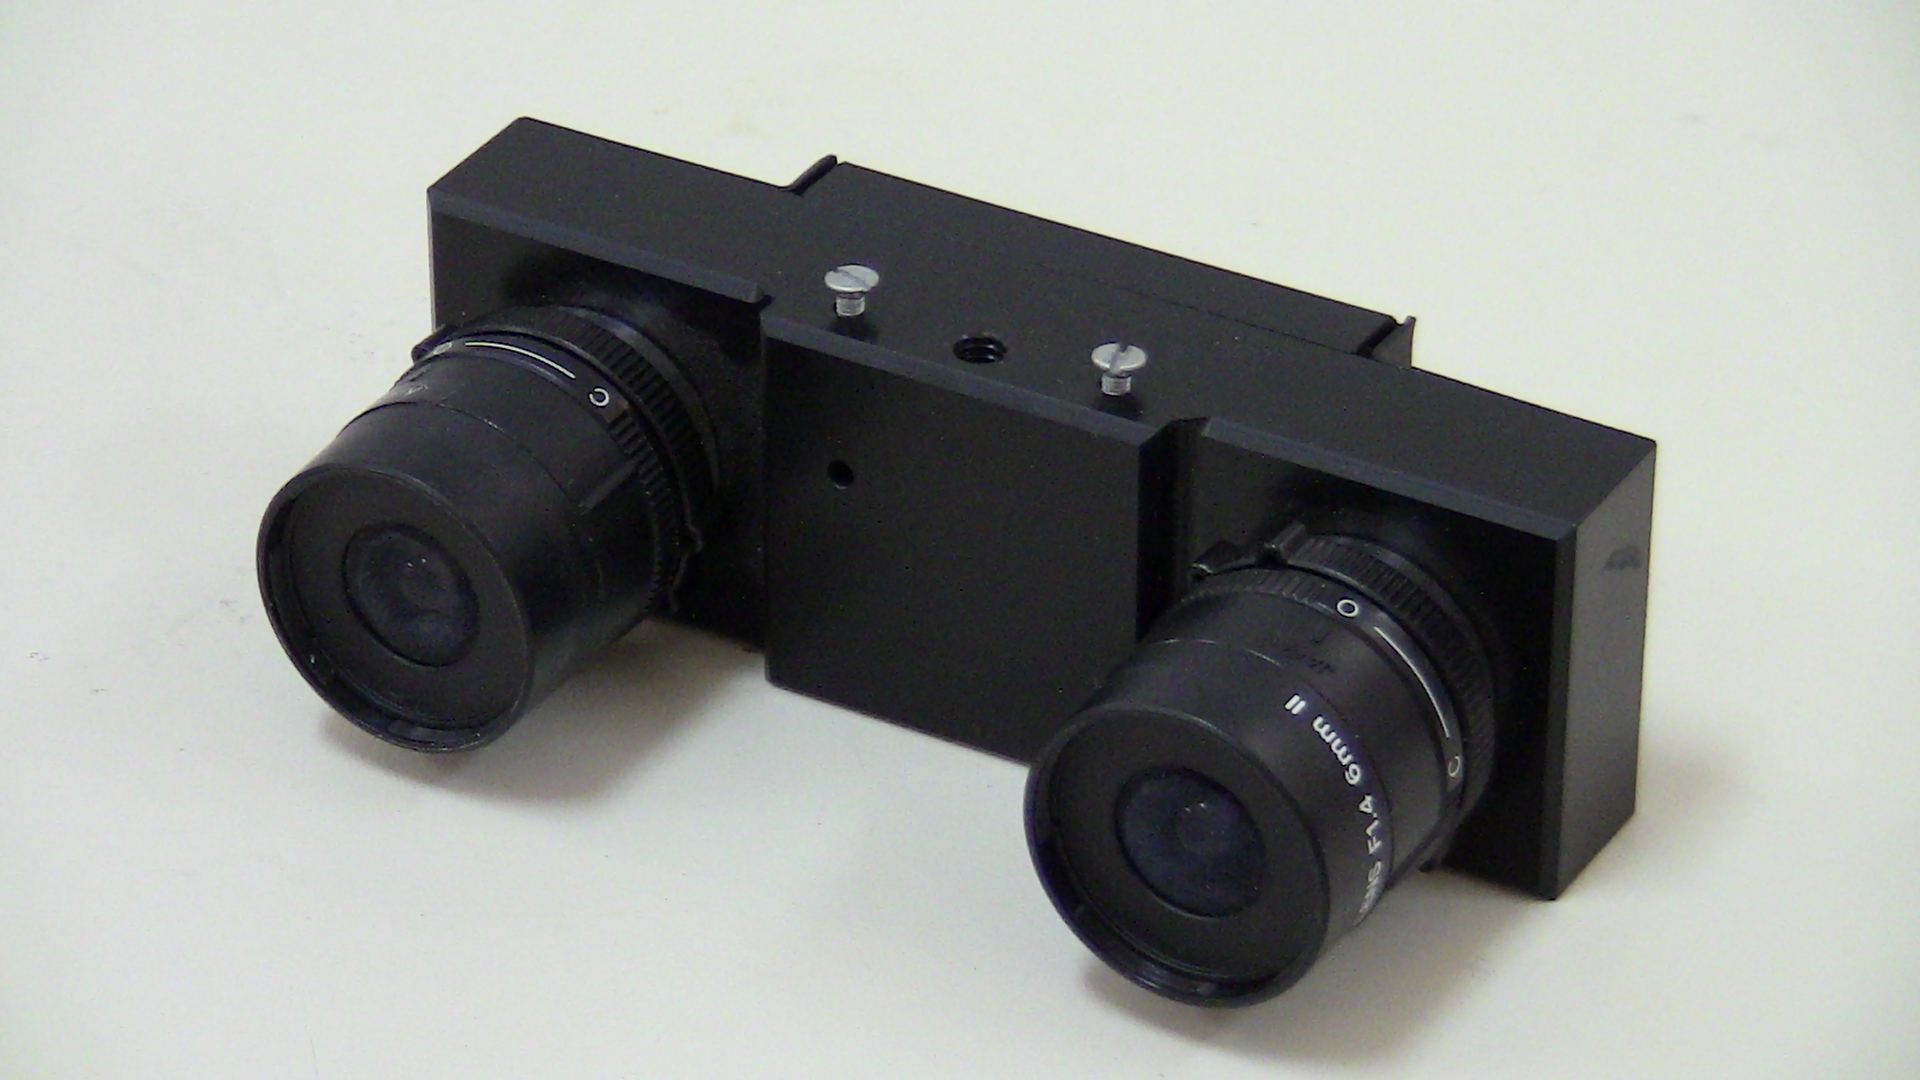
\includegraphics[width=0.4\textwidth]{figures/device_photos/camera.jpg}
\caption{Camera.}
\end{figure}

\begin{figure}[ht]
\centering
 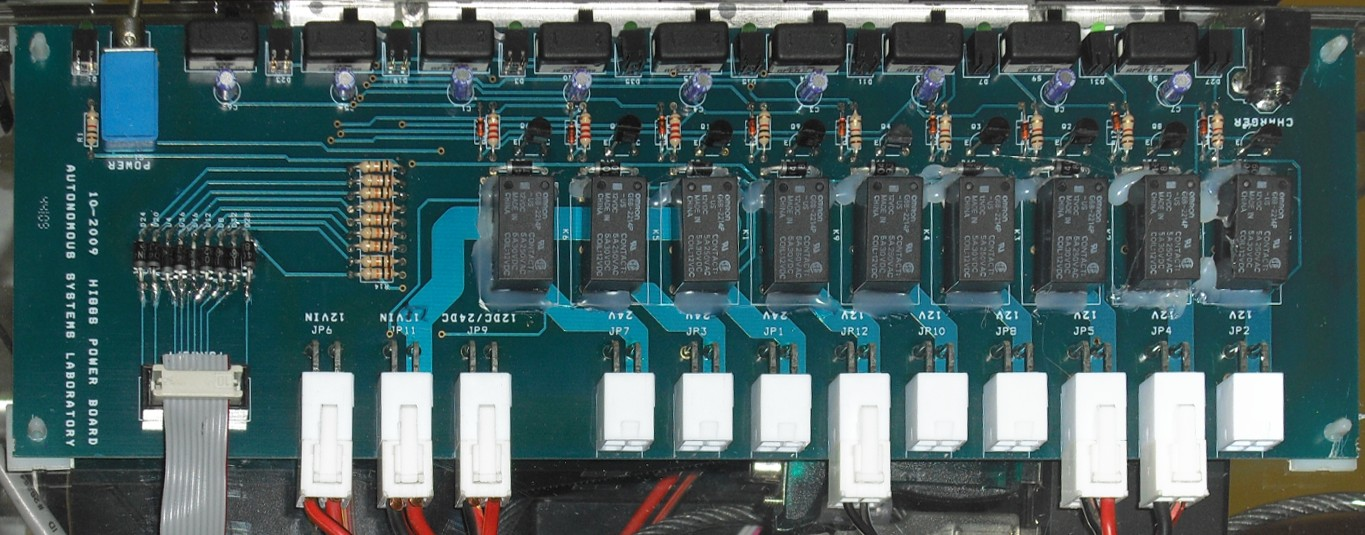
\includegraphics[width=0.5\textwidth]{figures/device_photos/powerboard.jpg}
\caption{Power board.}
\end{figure}

\begin{figure}[ht]
\centering
 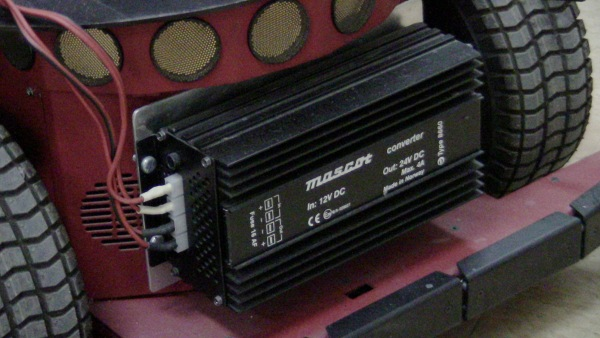
\includegraphics[width=0.5\textwidth]{figures/device_photos/converter.jpg}
\caption{12V to 24V converter.}
\end{figure}

\begin{figure}[ht]
\centering
 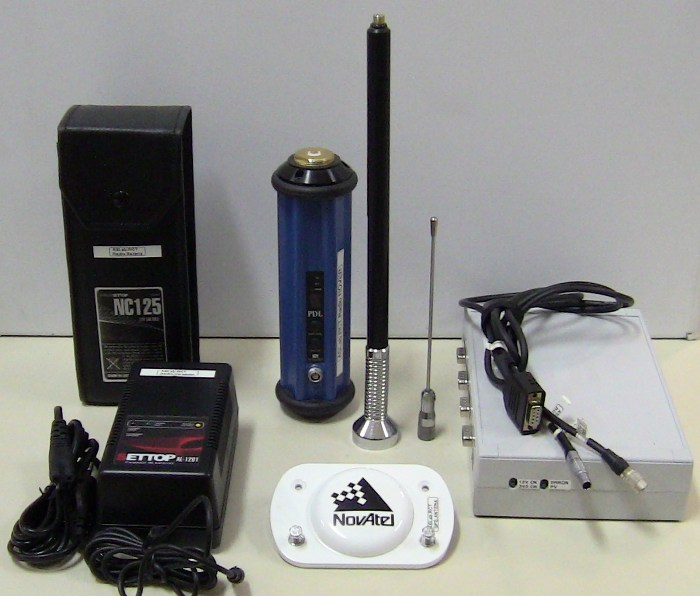
\includegraphics[width=0.6\textwidth]{figures/device_photos/gps_rover.jpg}
\caption{Differential GPS set. Rover station parts.}
\end{figure}

\begin{figure}[ht]
\centering
 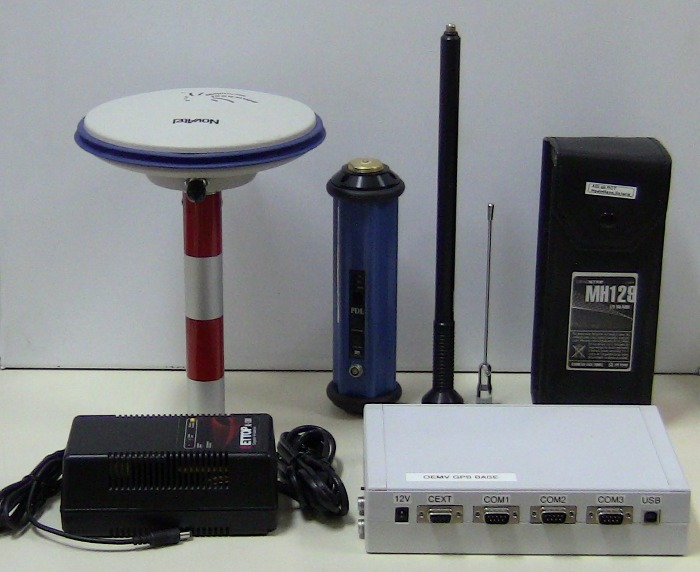
\includegraphics[width=0.6\textwidth]{figures/device_photos/gps_base.jpg}
\caption{Differential GPS set. Base station parts.}
\end{figure}

\begin{figure}[ht]
\centering
 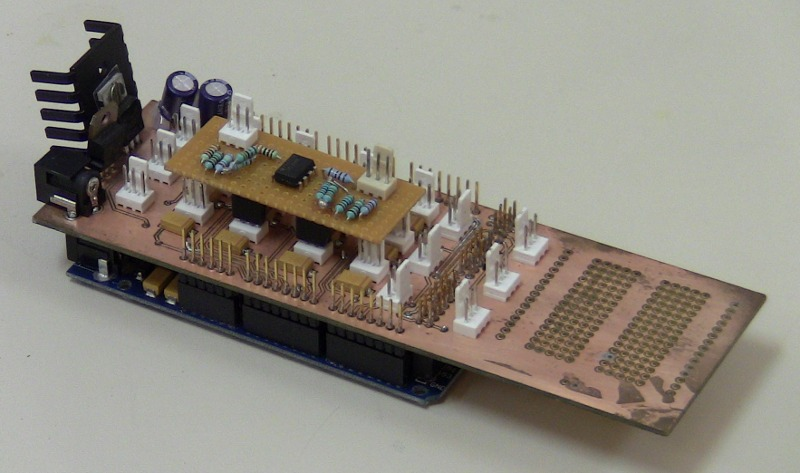
\includegraphics[width=0.5\textwidth]{figures/device_photos/ioiv.jpg}
\caption{Input/Output board: Arduino.}
\end{figure}

\begin{figure}[ht]
\centering
 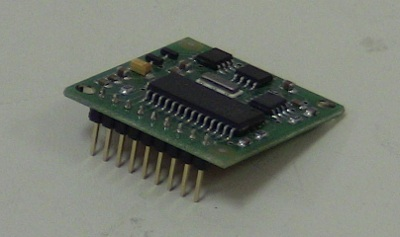
\includegraphics[width=0.3\textwidth]{figures/device_photos/compass.jpg}
\caption{Compass.}
\end{figure}

\begin{figure}[ht]
\centering
 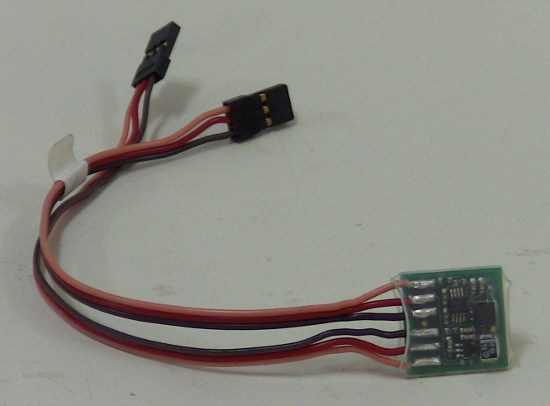
\includegraphics[width=0.4\textwidth]{figures/device_photos/accel.jpg}
\caption{Accelerometer.}
\end{figure}

\clearpage


\subsection{Data connection diagram}

\begin{figure}
\centering
 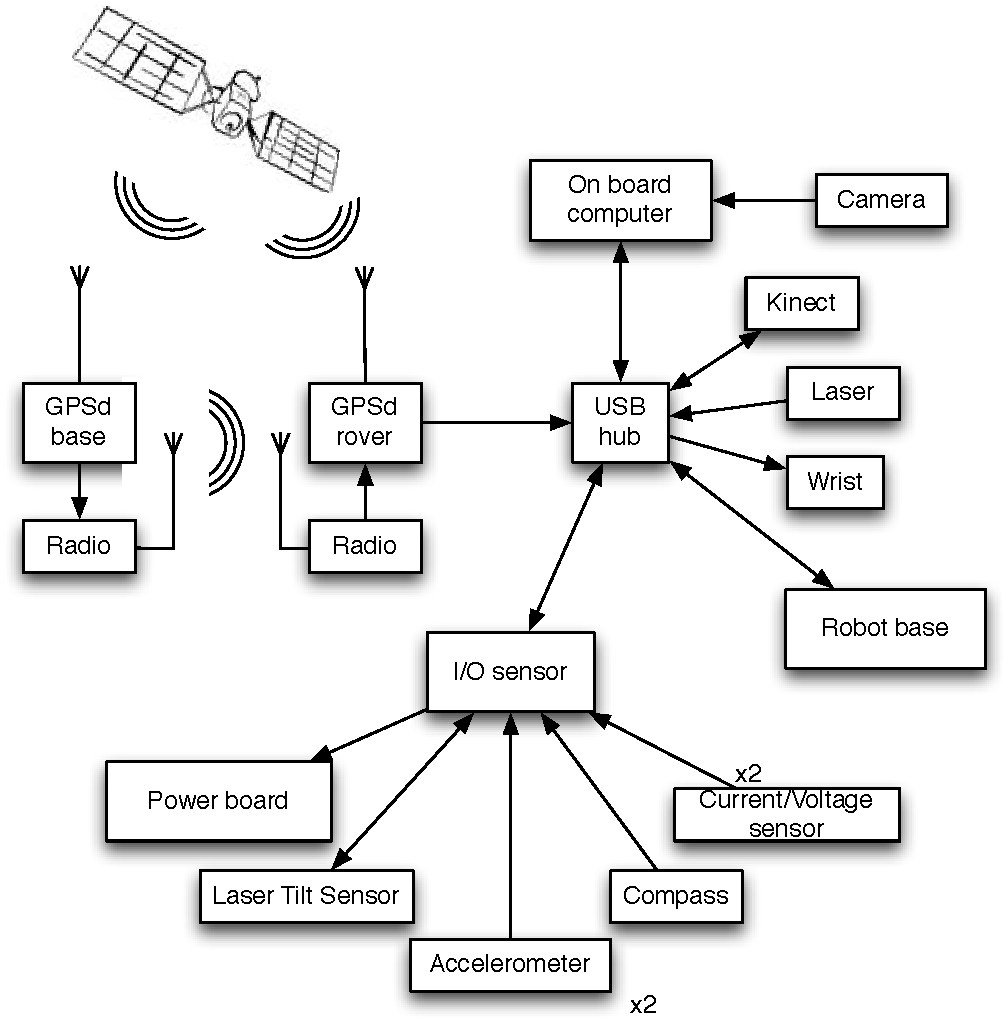
\includegraphics[width=\textwidth]{diagrams/RCT_datalines.pdf}
\caption{General data connection diagram}
\label{fig:higgs_data_connections}
\end{figure}

Arrows indicate the direction of valuable information flow.


\section{Basic maintenance}
\label{sec:usermanual_maintenance}

There is little maintenance to do with the robot. The batteries are the most important matter to be aware, followed
by the wheels.

\subsection{Wheels}
Once every two months or so, the wheels will loose pressure
and they must be inflated evenly, this way the odometry will not loose precision. It can be noticed
when the wheels have deinflated by looking to the tread pattern: Two separate bands of moist will indicate underinflation,
one on the middle overinflation, and correct inflation when moist is evenly distributed. There is a manual pump with
manometer in the ``sala F'' closet.

\subsection{Battery management}
The robot has 3 battery packages. One of them is inside the Pioneer2AT8, the other one powers the radio receiver
for the differential GPS and the laptop has its own.

\subsubsection{Robot base batteries}
There are three lead battery packages inside the Pioneer2AT8 that powers the motors, the internal electronics and
the external power board. To access them, lift the small black lever on the back side of the robot and turn it to the left.
This will loosen the battery door. Open it to 135$^{\circ}$. You may have to pull the door up to get the door over the
bump sensors. Once it is open, pull the batteries with the black sucker, or carefully with the hands do not get yourself
pinched. When inserting the new batteries, remember that \textbf{the battery terminals go last}. Failure to introduce
them correctly will cause short circuits and damage the electronics.

\begin{figure}[ht]
\centering
 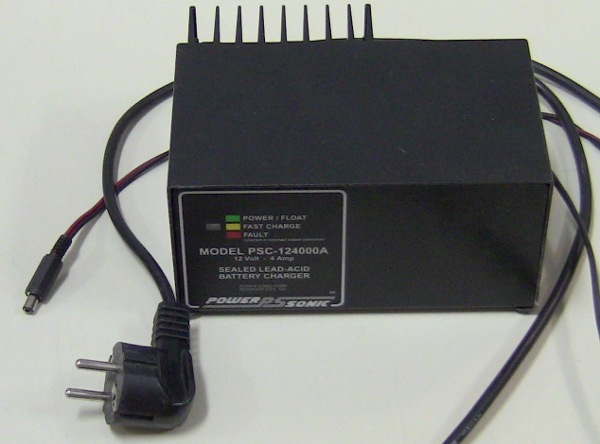
\includegraphics[width=0.6\textwidth]{figures/device_photos/rover_charger.jpg}
\caption{Robot base charger.}
\label{fig:base_battery_charger}
\end{figure}

Recommended voltage when using the batteries is between 11.5V and 12.5V. If the batteries are too low the robot
will indicate it with continuous short beeps. You can check the battery status through the battery LED in the
Pioneer2AT8 panel: Green when fully charge through orange downto 11.5V, finally red. You may find more information in the manual of the Pioneer2AT8 To keep the batteries in good
conditions, do not discharge them completely. Doing so will decrease the charge capacity. It is better to
fully charge them after each use.

To charge the batteries, connect the charger to the robot through the power jack connector to the
left of the battery door. Its charger is model PSC-124000A and is shown in figure \ref{fig:base_battery_charger}. You may leave the charger connected
for as long as you want, but remember to \textbf{switch off the robot after use}, as electricity in the
laboratory is turned off and the robot will fully discharge the batteries in this time, damaging them.

\subsubsection{GPSD radio battery}
There are two radio batteries, one for the GPS base station and the other for the GPS mobile station. Both batteries
are interchangeable, and are 8x9x23cm in size with a black leather cover.
Ni-MH batteries have memory effect, so you must discharge them completely before charging them again.
There are two chargers. you may found them in the yellow suitcase in the ``F room'' or in a white long box next to
the suitcase. Remember that the ``F room'' is the name for the ASLab cabinet in the computer rack room.
To charge it, open the battery tab and connect the charger. Press the button for discharging it fully, then wait until the
charger finishes the operation. Detailed instructions are printed on the charger. 

\begin{figure}[ht]
\centering
 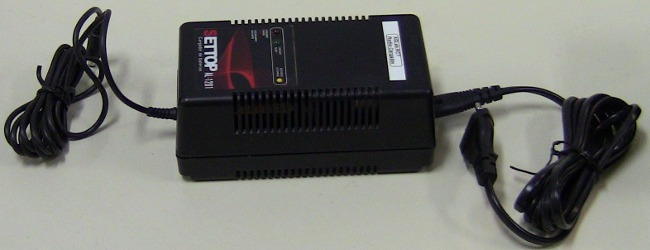
\includegraphics[width=0.7\textwidth]{figures/device_photos/gps_charger.jpg}
\caption{GPSD radio charger.}
\end{figure}

\subsubsection{VAIO laptop battery}
The VAIO laptop manages automatically its own battery. You may check its status with the command
\texttt{acpi -b} when running a UNIX based OS. On linux RTAI, ACPI is not supported by the kernel and it will not work so this command
is unavailable.

\begin{figure}[ht]
\centering
 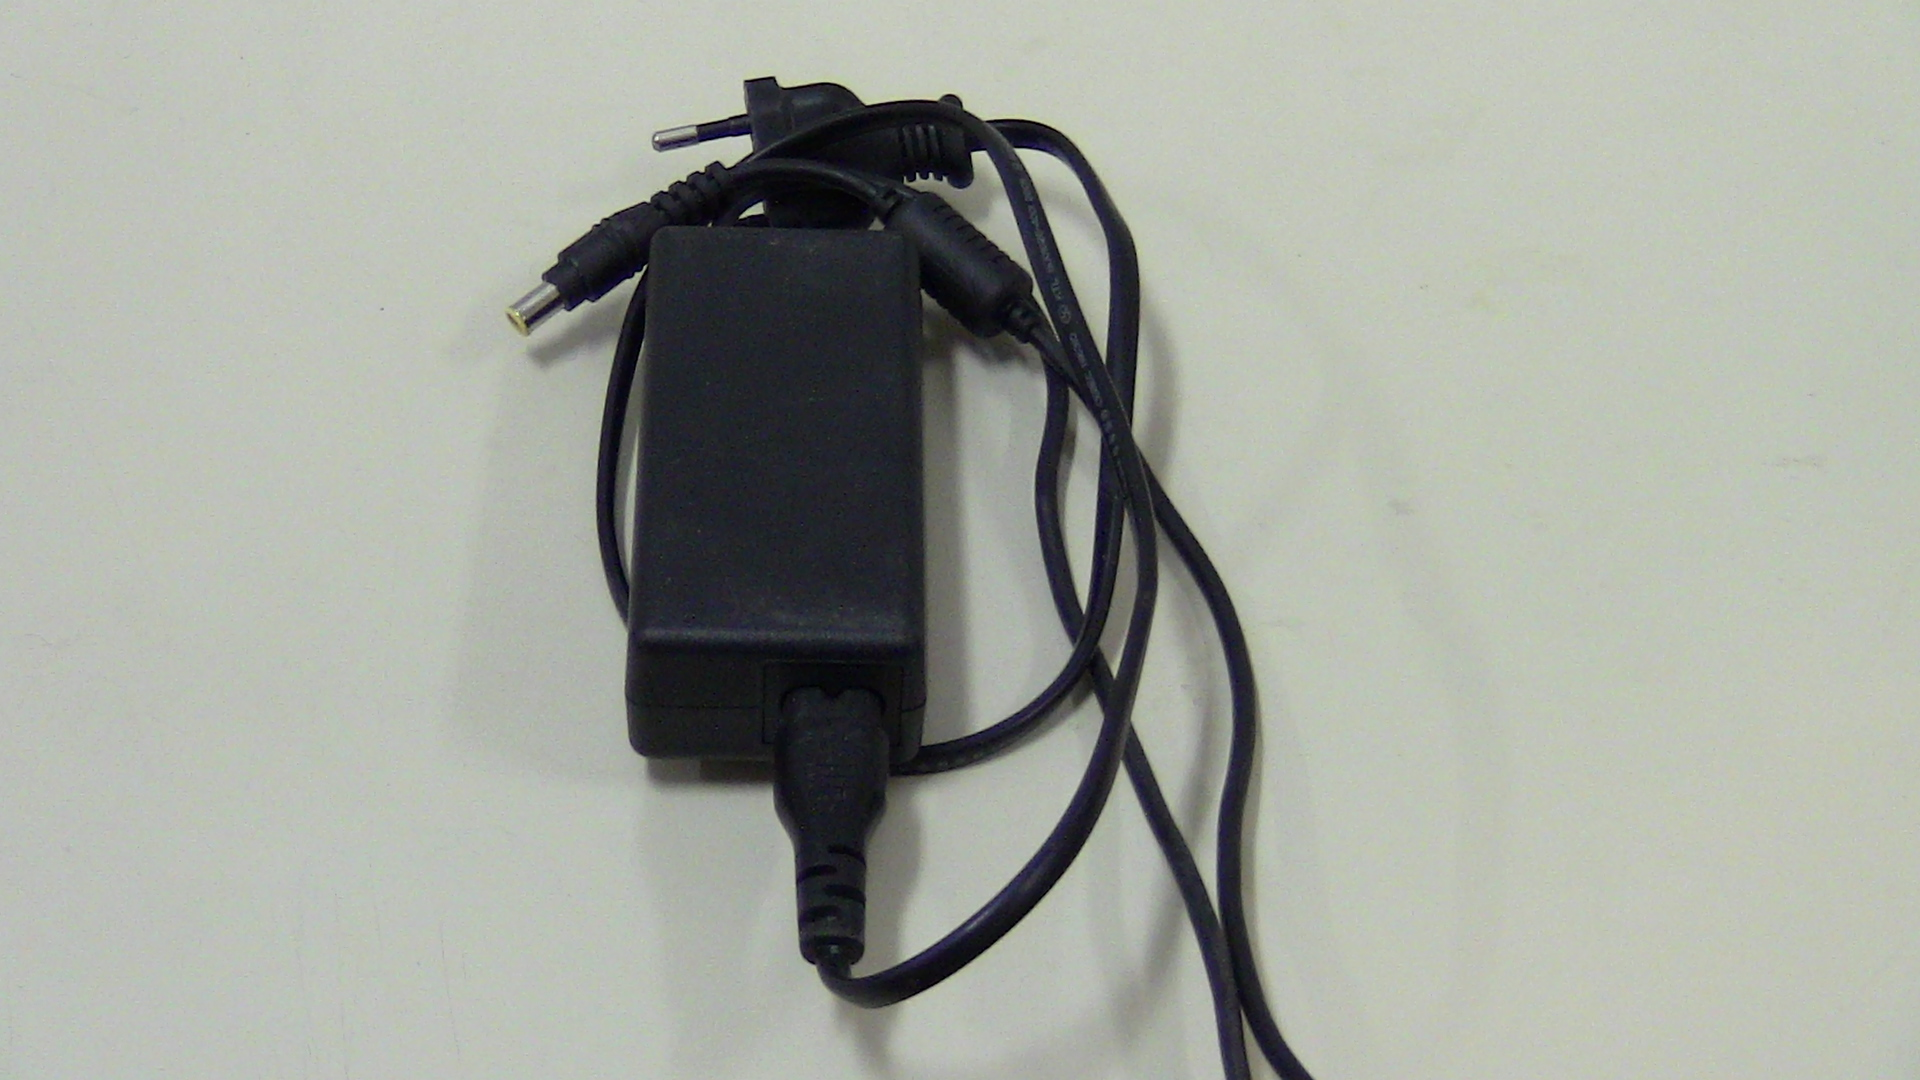
\includegraphics[width=0.7\textwidth]{figures/device_photos/vaio_charger.jpg}
\caption{VAIO laptop charger.}
\end{figure}

\subsection{Diagnostics}

\subsubsection{Power}
There are several indicators of malfunction that can ve verified in case the robot does not work properly.
In the first place, look for correct power in each device. This is how you can check it:
\begin{description}
 \item[Pioneer2AT] There is a red LED inside the Pioneer when it is powered, but can only be verified
indirectly through reflections in the methacrylate structure that covers the top hole of the base.
Alternatively, There is a dedicated red LED for this purpose in the Control Panel with the label \textit{PWR}.
\item[Laptop] The VAIO laptop lights a green LED when it is on.
\item[Laser] When it is powered on, a green LED or two orange and red LEDs will be lighted in the front of the
laser device. Green means powered and prepared, orange and red means powered and initializing.
\item[Arduino] When it is powered a little orange LED can be find behind the USB connector. A fast sanity check
is to power the arduino and the servo. If everything is OK, the Laser will rotate to look upwards in a small angle.
\item[Wrist] There is no way to verify this device externally. However, it is quite robust and will normally work
as supposed to. If everything is running ok, it will make a little calibration
movement on startup.
\item[Camera] Depends on the camera used. The black stereoscopic one has a red LED that blinks when the driver is
reading it and the Minoru3D lights up in white when the driver is reading it.
\item[GPS] There are two LEDs on the side. One of them indicates that power is OK and the other lights when enough satellites for position calculation are being tracked.
\item[Power Board] There is a green LED for the general switch and one for each device.
 \end{description}




\section{Setting up the system}
\label{sec:usermanual_setup}

Preparing the robot for operation is easy. Power it on and all systems will start automatically.
On next sections it will be discussed how to command it.

\subsection{Powering the robot}

There are three switches that must be turned on to enable the robot with full capabilities. The first one is
at the back of the robot, next to the wheels. This switch powers the Pioneer2AT8 robot base and the power board.
The power board has a general switch for all 6V and 12V devices and one more for each of these devices for manual disabling. The
power board is placed between the two big methacrylate structures. Each switch has a label with the device
it enables. The last device that should be powered is the VAIO laptop.

\textbf{Note:} The devices powered by the power board can be also disabled automatically by the
Arduino. When the Arduino is not correctly powered on, the voltage levels at its pins are undefined, and
may disable the power to some devices. Be sure to \textbf{power the arduino if you} are going to \textbf{use any other device
from the power board}.

Only the laptop is mandatory to power on. The other switches may stay off if you are not going to use the device
associated to that switch. However you will have to start at least one device to make it useful.

The Arduino does not disable any device by default.
Both the manual switches and the Arduino may force the shutdown of any device, so to use a device,
be sure that none of them disables it. The automatic switches are remotely controlled through the Arduino module.

\begin{figure}
\centering
 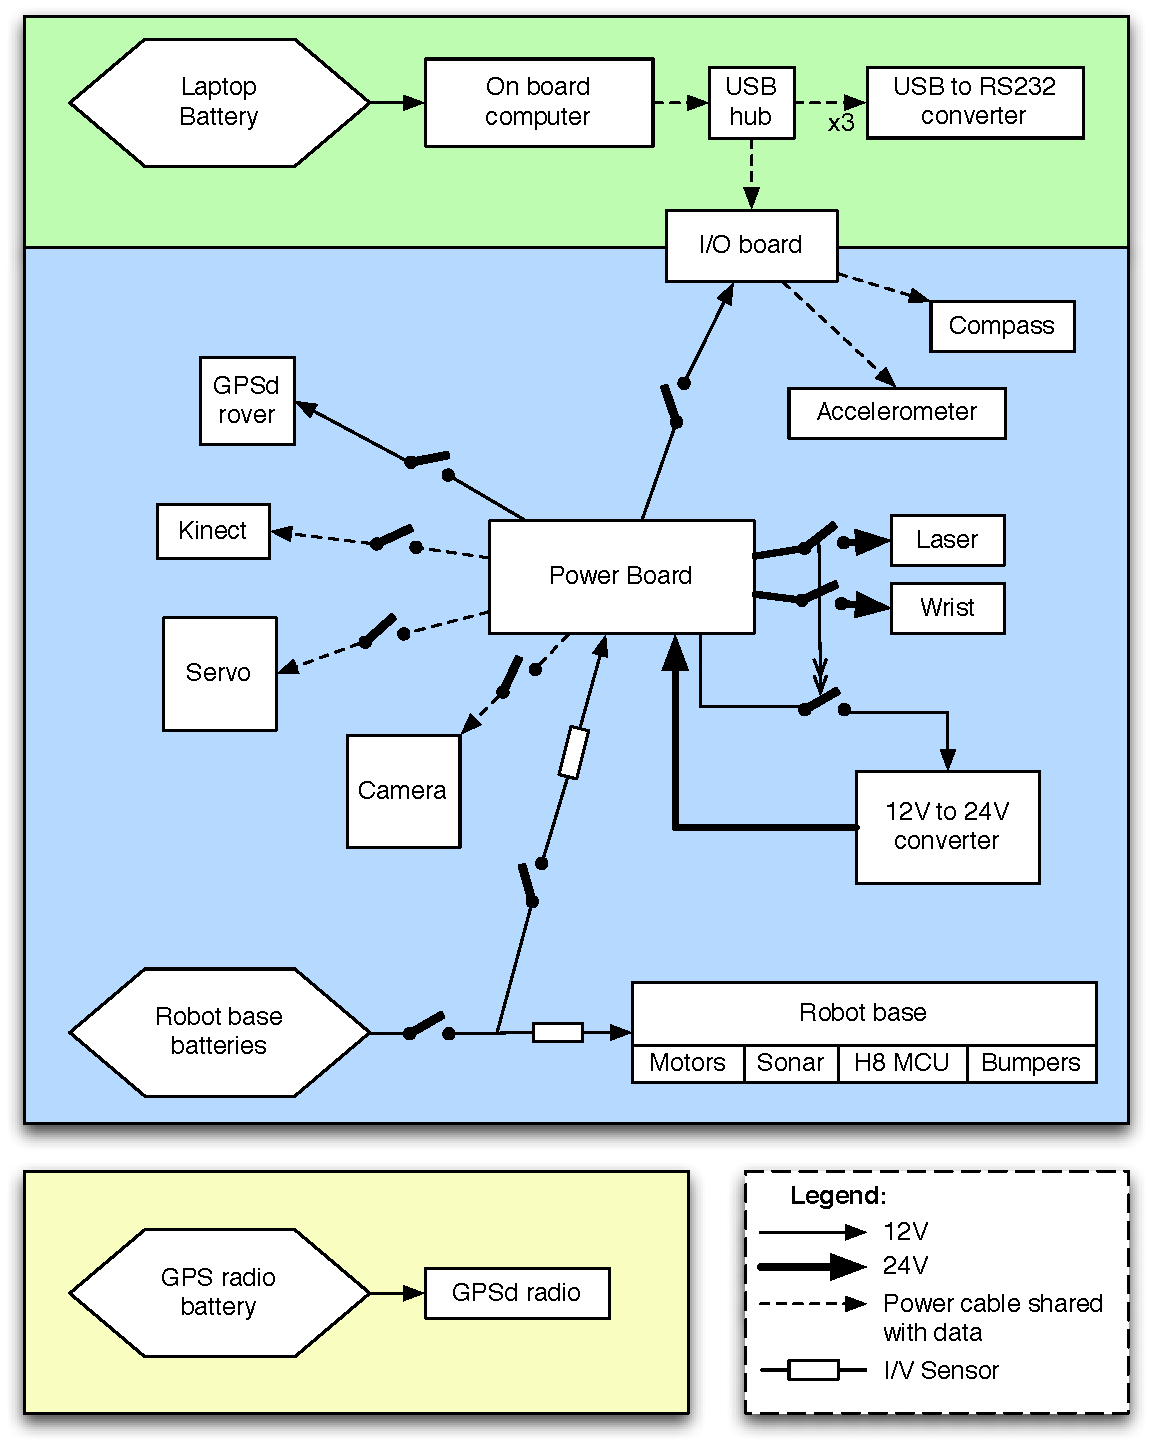
\includegraphics[width=1.1\textwidth]{diagrams/RCT_powerlines.pdf}
\caption{General power connection diagram}
\label{fig:higgs_power_connections}
\end{figure}



\section{Operating the robot}
\label{sec:usermanual_operating}

\subsection{Booting the onboard computer and choosing the OS}

The onboard computer has several operating systems installed:
\begin{description} 
 \item[WindRiver OS] \texttt{/dev/sda1} (1GB). This was once used as a testbench for the WindRiver OS. It is several years old
and is not used any more.
 \item[Windows XP Professional] \texttt{/dev/sda2} (25GB). The original Windows OS prepackaged with the laptop. The NovAtel GPSD
utilities have been installed here for quick GPS diagnostics.
 \item[Ubuntu 10.04 Long Term Service] \texttt{/dev/sda3} (14GB). This is the current
   working environment, with Real Time Application Interface (RTAI) kernel.
 \item[Fedora 13] \texttt{/dev/sda5 (29GB)}. Has the previous working environment, with CORBA modules set up and relying on the CORBA NameService in the old onboard computer. It aldo has a custom driver for supporting the FireWire camera.
 \item[Swap partition] /dev/sda6 (100MB).
 \end{description}
On bootup there is a selection of the operating system to start. It includes Ubuntu with and without real time kernel,
a RAM memory test and the other three OSs. The default OS is Ubuntu with the RTAI kernel.
Note that only the current working OS, that is, the Ubuntu with RTAI kernel, is documented here.
The other operating systems are old but kept for backup and compatibility with old software.

\subsubsection{Shutting down.}
The correct procedure to shut down the onboard computer is to log in as root and request shutdown:
\begin{verbatim}
root@higgs2:/root# halt
\end{verbatim}
Forcing instant shutdown using the power button is not recommended, however, normally there has been no problem with the OS afterwards.

\subsection{Loggin in to the onboard computer through SSH}

The Secure SHell server is run in the onboard computer by default and open to everyone that has a user account
or the root password. The root password is the same as the root password for all the computers in the laboratory.
Ask your tutor for a local account on higgs or the root password. Access can be obtained by opening a terminal
and executing the command
\begin{verbatim}
your-pc:/$ ssh account_in_higgs@higgs2
\end{verbatim} 
and root access by changing \texttt{account\_in\_higgs} with \texttt{root} or changing user to root after logging in..
If you want to execute programs that use a graphical interface, create a ssh tunnel for X with the option \texttt{-X}:
\begin{verbatim}
your-pc:/$ ssh -X account_in_higgs@higgs2
\end{verbatim}
This way the program will execute in the onboard computer and display in your local screen remotely.
In case you get this error while trying to connect:
\begin{verbatim}
 ssh: Could not resolve hostname higgs2:\
	Name or service not known
\end{verbatim}
then you have a problem with the name resolution on your computer. Copy these lines to your \texttt{/etc/hosts}
as root to solve it:
\begin{verbatim}
138.100.76.251  sagan.aslab.upm.es		sagan
138.100.76.247	higgs.disam.etsii.upm.es	higgs
138.100.76.246	higgs2.disam.etsii.upm.es	higgs2
\end{verbatim}
Now your computer knows how to translate the hostnames of the laboratory to IP's.
Alternatively, if in a rush substitute \texttt{higgs2} with its IP, as in
\begin{verbatim}
your-pc:/$ ssh local_account@138.100.76.246
\end{verbatim} 

The machine with name \texttt{higgs} corresponds to the old on board computer which was embedded inside the robot base.

Once logged in to higgs2, applications can be run as in a standard linux distribution.
Linux RTAI runs a normal kernel with standard functionality ontop of the realtime features.
For using realtime, the programs must be loaded directly into the kernel as modules. All other programs 
run in soft real time.

On bootup, the onboard computer will connect automatically to the wireless
accesspoint \texttt{aslab\_wireless}.
This accesspoint is in the same network as the  other computers. The connection is configured using the ESSID of the wi-fi hotspot and the MAC address too.


\section{Testing the CORBA modules}

The CORBA servants\footnote{A CORBA servant is an executables that provides the functionality described by the IDL file that implements.} access the NameService to publish their services\footnote{If appropriate module is installed and running.}. The table \ref{tab:names_ID_CORBA} shows the ``\texttt{id}'''s used by each module, being the ``\texttt{kind}'' parameter empty for all of them.

\begin{table}
\begin{center}
\begin{tabular}{ccc}
\textbf{Description} & \textbf{IDL} & \textbf{Name Service ID} \\ 
\hline
Camera & Camera.idl & CAMERA \\ 
I/O Board & Arduino.idl & Arduino \\ 
Robot base & Pioneer2AT.idl & PIONEER \\ 
Wrist & wrist.idl & wrist \\ 
Battery Model & BatteryModel.idl & BatteryModel \\ 
Current Monitor & BatteryModel.idl & CurrentAverage \\ 
Laser & Laser.idl & LASCOR \\ 
GPS & gps.idl & GPS
\end{tabular}
\end{center}
\caption{Names of the CORBA objects registered in the NameServer.}
\label{tab:names_ID_CORBA}
\end{table} 

\subsection{Subversion.}
The device modules have test programs that can be run either locally from the onboard computer or remotely
without needing to log in. This section and the next one are a quick guide for reconfiguring and troubleshooting easy problems with the devices. Any problem not solved here requires further understanding of the robot software mechanisms and are described in the developer manual.

The first thing to do is download the source code. Supposing you already have installed the necessary programs and libraries, type
\begin{verbatim}
svn co svn+ssh://sagan/home/svn_repositories/Higgs
\end{verbatim}
to check out the source. Again, replace \verb"sagan" with 138.100.76.251 if your hosts.conf is not correctly configured and prepend it with your user name and an @ if your server user is not the same as the local user.

There is a second repository with modules and code that have not yet been ported to the new CMake - subversion schema.
\begin{verbatim}
svn co svn+ssh://sagan/home/svn_root[/Higgs]
\end{verbatim}
If you need to search for older code there is also an obsolete CVS repository.

\subsection{Subversion directory hierarchy}

Once finished, three directories will be available:
\begin{description}
\item[\texttt{trunk}] The latest code available using the technology currently in development in the robot, which is ROS at the time of this writing.
\item[\texttt{branches}] Alternative code using other technologies, which currently is only CORBA.
\item[\texttt{docs}] The source code of this document.
\end{description}

This is the resumed directory tree inside \texttt{branches/CORBA}:
\begin{verbatim}
code
|-- LowLevelControl
|-- WorldModel
|-- batteries
|-- control_libraries
|-- devices
|   |-- arduino
|   |-- camera
|   |-- gps
|   |-- laser
|   |-- vaio_tools
|   `-- wrist
|-- idl
`-- lib
\end{verbatim}
The directories to consider when programming new clients are:
\begin{description}
\item[\texttt{code/idl}] Contains the IDL definition files of all the modules necesary for controlling the robot. You may open it for accessing the documentation for the interfaces and you will have to link to it for generating the stubs and skeletons.
\item[\texttt{lib}] C++ macro and CMake files (See section \ref{ssec:cmake}) for fast client development.
\end{description}


\subsection{Checking the environment for starting test programs.}

\subsubsection{Configuration files}

The next sections describe how to run the test programs contained in the CORBA branch for testing the devices.
The server is the onboard computer and the clients may refer both to the onboard computer or any other remote computer,
wherever the client software is running. Typically this computer will be from where the human operator is testing the modules.

Before running the test clients the configuration files must have been installed for proper operation.
Clients only need one configuration file:
\begin{verbatim}
/etc/higgs/nameservice.ip
\end{verbatim}
containing the address and port of the Naming Service that the servants are using for publishing themselves:
\begin{verbatim}
higgs2:9876
\end{verbatim}

\subsubsection{Configuring serial port links}
\label{sec:serial_links}

On the server side there are a few more entries inside \texttt{/etc/higgs}, the most important one for configuration issues being \texttt{devices}. This directory contains soft links to the character devices that represent the USB to RS-232 converters in \texttt{/dev}. The servants open these files instead of the real devices so they can be reconfigured without having to recompile. Usually you will modify these links when swapping the serial cables of the devices or changing the arrangement of the USB to serial converters. Knowing which device file goes with which device is a matter of trial and error, starting the servants and testing wether they started or not. See \ref{sec:user_log} for more information on servant logging.


\subsubsection{Starting and stopping the CORBA servants}
The servants use upstart, the standard utility in Ubuntu for booting the system and running the daemons.
You may start or stop the servants in case you need the correspondant devices, i.e. when using the laser and the robot base with ROS, or they are not automatically started on boot.

To start a servant use:
\begin{verbatim}
$ start higgs_device
\end{verbatim}
and to stop it,
\begin{verbatim}
$ stop higgs_device
\end{verbatim}
where \verb"device" is one of laser, wrist, gps, arduino, pioneer or any other available CORBA servant.

There is one more daemon, the CORBA Naming Service, which opens the port 9876, It is always running and does not interfere with the devices.

\subsubsection{Logs and troubleshooting}
\label{sec:user_log}
Servants print their output to a log file in the on board computer placed at \texttt{/var/log/higgs}. You will have to consult these for debugging problems with the servants such as not starting, setting the device file and checking overall status.

\subsection{I/O board}
The next procedure is standard on all modules.
Enter the directory \\ \texttt{\$(HIGGS\_ROOT)/branches/CORBA/code/devices/arduino/client}.\\
Be sure to have the complete source tree, at least the code subdirectory, as many methods rely on files situated back in the tree.
Run:
\begin{verbatim}
cmake .; make
\end{verbatim}
This will generate the CORBA stubs and headers and then compile the client code. The binary \texttt{arduino\_client} will appear. Run it to read the parameters of the devices attached to the I\/O board and set or reset some of the devices.

\subsection{GPSd}
You may want to test the full GPSd equipment with differential corrections or only the rover part. The differential readings may not work in the campus because of interferences in the environment that blocks radio communications between the base station and the rover.

\subsubsection{Rover}
In the first place check that
 the serial cables are correctly installed. The USB to RS232 converter should be attached to the port labeled COM1 in the GPS electronics box. Turn on the GPS switch on the powerboard. Now to the software part: Go to \\ \texttt{\$(HIGGS\_ROOT)/branches/CORBA/code/devices/gps/src} and run \\
\texttt{cmake .; make}. Run \texttt{gps\_client}. A command line menu will be printed form where you can check the satellites used in the solution, the current position and speed, the standard deviation for the position and the type of differential corrections used, if any.
This will give you the GPS calculations without differential corrections. Set up the base station to improve precision.

\subsubsection{Receiving differential corrections from the base station}
The software part is the same as in the Rover part, with the standard deviation reducing to 0.02m or so if the differential correction is working. The preparation of the base station follows.

Go to the ASLab closet and locate a yellow bag. Take out the black leather battery, the blue radio transmitter with the antenna, the white box housing the electronics and the cables. The GPS antenna is located on the roof with the coaxial cable hanging down the facade to the back of the room where Higgs lives. Open a window and take it inside. Beware of your workmates in winter! Connect it to the electronics box. Power the electronics box with 12V, for example using Higgs charger, and the radio transmitter to the battery pack using the appropriate cable. Finally connect the electronics box to the battery pack with the serial terminal attached to COM2. The battery pack is internally wired to connect the serial data and the power to the cable attached to the serial transmitter. Press power in the serial transmitter. After a few minutes, the Tx led should start blinking every second. This is the indication that the differential readings are being transmitted.

In the \textbf{rover part}, attach the three terminal cable to the blue radio receiver, the battery pack and the COM2 port in the rover GPS electronics box. Press the power button in the radio receiver and proceed as in the rover section.

\subsection{Laser}
Procedure is similar to the I/O board one. Go to \\ \texttt{\$(HIGGS\_ROOT)/branches/CORBA/code/devices/laser/src}
and \\ \texttt{cmake .; make}. \texttt{laser\_client} will be generated. Power the laser in the robot, wait for it to go green and some more seconds for the laser servant to start up, and run the client. A list with the distances of the latest reading will be printed to the console.

\subsection{Wrist}
Again, the procedure is similar, only in this case the device is an actuator and so does not give sensor readings but obeys commands. Turn on the switch for the wrist and wait for a little calibration movement that indicates that it is ready. It will move to the reset position if not there before the calibration.
Go to \\ \texttt{\$(HIGGS\_ROOT)/branches/CORBA/code/devices/wrist/src}. \\ Two clients will appear. The first of them, \texttt{wrist\_client}, will move the two axis with incremental span around ten times then stop. The second one, \\ \texttt{wrist\_client\_mouse\_grab}, will let you control the two axis with the mouse. Once running, take the pointer to the center of the window to move the wrist to the starting position, then slowly move the pointer and the wrist will follow it. The range of movements is limited by the servant for secure operation whatever the input is. However, the batteries and converter may not be able to provide the required power if too fast movements are requested.

\subsection{Robot base}
TODO

\section{Developing a client}
\label{sec:dev_client}


\subsection{ASLab client utility functions for CORBA}
The methods for initializing the CORBA infrastructure and getting the object references is quite complicated and always the same. The file \\
\texttt{code/lib/CORBA\_utils.h} contains C++ macros that ease the procedures for setting up a client, managing the errors, reading the object references from the nameserver and configuring itself for reaching that nameserver.

The typical client would be something like:

\begin{verbatim}
#include <iostream>
#include "implementationC.h"
#include "CosNamingC.h"
#include "Higgs/branches/CORBA/code/lib/CORBA_utils.h"

int main(int argc, char* argv[])
{
    CORBA_BEGIN_CLIENT(argc, argv);
    CORBA_GET_REFERENCE(module::implementation, impl, "IMPL");

    impl->do_things();

    CORBA_END_CLIENT;
    return 0;
}
\end{verbatim} 

With the correct route to \texttt{CORBA\_utils.h}. The arguments for \texttt{CORBA\_GET\_REFERENCE()} are:
\begin{enumerate}
\item \texttt{module::implementation} The type of the object to fetch.
\item \texttt{impl} The identificator desired for the reference. It should not be defined nor declared, it is done inside the macro. Remember that references are used as pointers.
\item \texttt{"IMPL"} String with the name that the object is registered in the NameServer.
\end{enumerate}




\subsection{CMake}
\label{ssec:cmake}
It is encouraged to use CMake as the tool for managing the compilation of the proyects. There is a sample CMakeLists.txt in \texttt{Higgs/branches/CORBA/code/lib}  prepared for linking the CORBA libraries and generating the necessary dependencies for compiling. Substitute \texttt{\_module} with the name of your module. The file \texttt{IDL\_command.cmake} defines a macro for generating and managing the sources of the IDL interfaces. Include all interfaces that you need when calling the macro \texttt{MacroGenerateIDL}.
Use the command
\begin{verbatim}
SET(IDL_DIR path/to/idl)
\end{verbatim}
pointing to higgs' idl definition files to tell the macro where to find them.


